\section{Analyse der Ergebnisse}
\label{sec:gesamtanalyse}
\todo{Zahlen auf Richtigkeit prüfen}
\todo{Zahlen auf einheitliche Schreibweise prüfen}
\todo{Begrifflichkeit Cluster oder Region. Und schreiben wir die Nummern dahinter aus oder nicht?}
\todo{STRG+F Kavernen, Euro, PV, CO2, C02}
\todo{Groß/Kleinschreibung Onshore, Offshore \- Achtung Satzanfänge!}

Im Folgenden erfolgt eine Gesamtbewertung für die einzelnen CO\textsubscript{2}-Restriktionen unter Berücksichtigung der jeweiligen Komponenten des Energiesystems. Im anschließenden Kapitel \ref{sec:reduktionsfaelle} wird dann noch mal die herausstechende Besonderheit je Reduktionsfall betrachtet. 

\subsection{Energiegewinnung}
Die unterschiedlichen Reduktionsziele stellen den Bedarf der Energieerzeugung aus erneuerbaren Energien dar. Insbesondere die Gewinnung aus Wind Onshore, Wind Offshore und Photovoltaik steigen signifikant, wobei der Anteil an Wind Onshore kleiner ausfällt als die beiden anderen genannten. 

Betrachtet man die installierte Leistung für Wind Onshore für den 75 \% Reduktionsfall liegt der Anteil bei 36 GW und reduziert sich bei 80 \% auf 23 GW. Ab einer CO\textsubscript{2}-Reduktion von 85 \% nimmt der Anteil wieder zu und steigt im 100 \% Szenario auf 44 GW. 
Dahingegen wird bei Wind Offshore ein signifikant steigender Anteil ermittelt. Im 75 \% Reduktionsfall beträgt dieser 48 GW und steigt auf 81 GW bei einem Reduktionsfall von 90 \%. Dieser Wert ist scheinbar das Kapazitätsmaximum und bleibt daher bis zum 100 \% Szenario konstant.

Ein besonders hoher Anstieg ist bei der Energiegewinnung aus PV festzustellen. Beträgt dieser im Szenario 75 \% noch 30 GW, steigt er bei allen weiteren Reduktionsfällen ab 85 \% überproportional bis hin zu 188 GW installierter Leistung.

\smallimage{Erzeugung_EE.png}{Installierte Kapazität der EE je Reduktionsfall}

Die Erdgasverstromung aus GuD-Kraftwerken erhält in den ersten beiden Reduktionsfällen noch eine unverzichtbare Rolle mit einem Anteil von 56 \% im 75 \% Fall und mit 47 \% im 80 \% Fall. Bei den weiteren CO\textsubscript{2} Reduktionszielen verringert sich der Anteil kontinuierlich, bis dieser bei einem CO\textsubscript{2}-neutralen Energiesystem vollständig verschwindet. Dies ist damit zu begründen, dass bei der Verbrennung von insbesondere Erdgas viel CO\textsubscript{2} freigesetzt wird und sich somit negativ auf die CO\textsubscript{2}-Bilanz auswirkt. Anstelle des Erdgases wird deshalb in den Fällen mit höheren CO\textsubscript{2} Reduktionszielen auf Biogasanlagen gesetzt, da dabei kein CO\textsubscript{2} freigesetzt wird. 


\subsection{Energieumwandlung}
Bei der Energieumwandlung wird die Elektrolyse als wesentliche und unverzichtbare Größe dargestellt. Dabei ist die Elektrolyse so bedeutsam, weil sie die einzige Möglichkeit ist, um Strom in Gas umzuwandeln und so langfristig zu speichern.

Im betrachteten Energiesystem bleibt der Wert für den Einsatz der Elektrolyse für die ersten drei Reduktionsfälle gleich hoch. Ein Anstieg tritt ab dem 90 \% Fall ein und verdeutlicht die Notwendigkeit zum Ausbau der Elektrolyseleistung. Mit steigenden Reduktionsfällen wird mehr Leistung in der Elektrolyse benötigt, um die Erzeugungsspitzen aus erneuerbaren Energien zu berücksichtigen und den Bedarf der Wasserstoffherstellung zu decken. 

\smallimage{Elektrolyse.png}{Verlauf der Kapazität der Elektrolyse über die einzelnen Reduktionsfälle hinweg}

In allen Szenarien der CO\textsubscript{2}-Reduktion befindet sich die größte Kapazität der Elektrolyse in Region 6. Dies lässt sich vermutlich damit erklären, dass nur in Region 6 die Stromerzeugung durch Wind Onshore stattfindet. Durch die Nähe von Erzeugern mit hohem Überschuss zu den Elektrolyseanlagen, kann der Strom direkt durch die Wasserstoffherstellung genutzt werden. In den Reduktionsfällen 75 \% und 80 \% ist Region 6 mit 11 GW die Einzige mit Elektrolyseanlagen.

In den Reduktionsfällen 85 \%, 90 \% und 95 \% gibt es zusätzlich eine Kapazität in Region 2. Die Investition in diese ist ähnlich zu erklären wie die Elektrolysenutzung in Region 6. Statt jedoch der Erzeugung aus Wind Onshore, hat die Region 2 die größte Erzeugung aus Wind Offshore.
Über die genannten Reduktionsfälle steigt dabei in beiden Regionen die Kapazität ähnlich stark an. 

In der 100 \%igen Reduktion von CO\textsubscript{2} sind für nahezu alle Regionen Elektrolyseanlagen vorgesehen. Lediglich Cluster 7 besitzt keine eigenen Anlagen und wird aus dem Pipelinenetz mit Wasserstoff versorgt. Die großen Kapazitäten liegen dabei weiterhin in Cluster 6 und 2.

\subsection{Energiespeicherung}
Die Energiespeicher erhalten bei steigenden Reduktionsfällen eine relevante Rolle. Der Bedarf resultiert aus dem notwendigen Ausbau der erneuerbaren Energien und der dazugehörigen Systemintegration. 
Dadurch können kurzfristige Übererzeugungen und Nachfrageschwankungen reguliert werden. 

In allen Szenarien ist ein Anstieg der Speichernutzung festzustellen. H\textsubscript{2}-Salzkavernen und Biogas Salzkavernen erhalten neben Batteriespeichern und Pumpspeicherkraftwerken eine neue wichtige Rolle. Die Pumpspeicher werden in allen Reduktionsfällen bis zum Kapazitätsmaximum ausgelastet, erhalten jedoch mit steigender Reduktion eine deutlich höhere Nutzung. 
Aufgrund des Gasimports werden die Kavernen bei geringen Reduktionsfällen nicht berücksichtigt. Mit steigendem Reduktionsfall werden größere Speicher jedoch erforderlich.

\smallimage{SpeicherDieSpeicher.png}{Verlauf der Speichernutzung}
\todo{Im Text verlinken}

Ein Batteriespeicher speichert Strom kurzfristig und muss deshalb die Kapazität haben, um große Strommengen auf einmal zu speichern. Durch die beschränkte Größe sind Batteriespeicher in jeder Region möglich und auch immer im Einsatz.
Im Vergleich zu Batteriespeicher sind Pumpspeicherkraftwerke größer, da sie mithilfe von Wassermengen Strom mittelfristig speichern können. Pumpspeicher sind in allen Regionen bis auf Region 7 im Einsatz.
Die Speicher, die langfristig speichern, sind Kavernen. Diese benötigen jedoch einen unterirdischen Hohlraum, der als Speicher dienen kann. Die Gegebenheiten für einen solchen Speicher sind also nicht überall einfach zu finden. Kavernenspeicher für Biogas gibt es in Region 1, 2, 3 und 5, während Kavernenspeicher für H\textsubscript{2} in Region 1, 2, 3, 5 und 6 angesiedelt sind. In einigen dieser Regionen wird Strom aus Windenergie erzeugt, sodass der Überschuss in Gas umgewandelt und direkt eingespeichert werden kann.


\subsection{Energieübertragung}
Mit steigendem Reduktionsfall verhält sich die Wasserstoffnutzung eher konstant. Schon im 75 \% Reduktionsfall wird eine installierte Leistung mit 29 GW berücksichtigt. Um die erforderliche Menge und somit die Nachfrage bedienen zu können, ist der Ausbau des Pipelinenetzes erforderlich. Im 95 \% Reduktionsfall beträgt die Spitzenleistung 31 GW. Ein Rückgang der Leistung simuliert der 100 \% Fall mit einem Wert von 19 GW. In dem Zusammenhang spielt die Sektorkopplung eine große Rolle, wenn im Energiemodell die Emissionsreduzierung im Fokus steht. 

Der Strom wird in Form von Wechselstrom (AC) oder Gleichstrom (DC) über Leitungen transportiert. Die Kapazität von diesen bleibt über alle Reduktionsfälle hinweg gleich. Zwar ist nicht jede Region mit Leitungen für AC mit allen anderen Regionen direkt verbunden, aber es sind alle angeschlossen. Bei den Leitungen für DC haben nur die Regionen 0, 2, 4 diese.

\begin{figure}[!h]
    \begin{minipage}[b]{.4\linewidth} 
       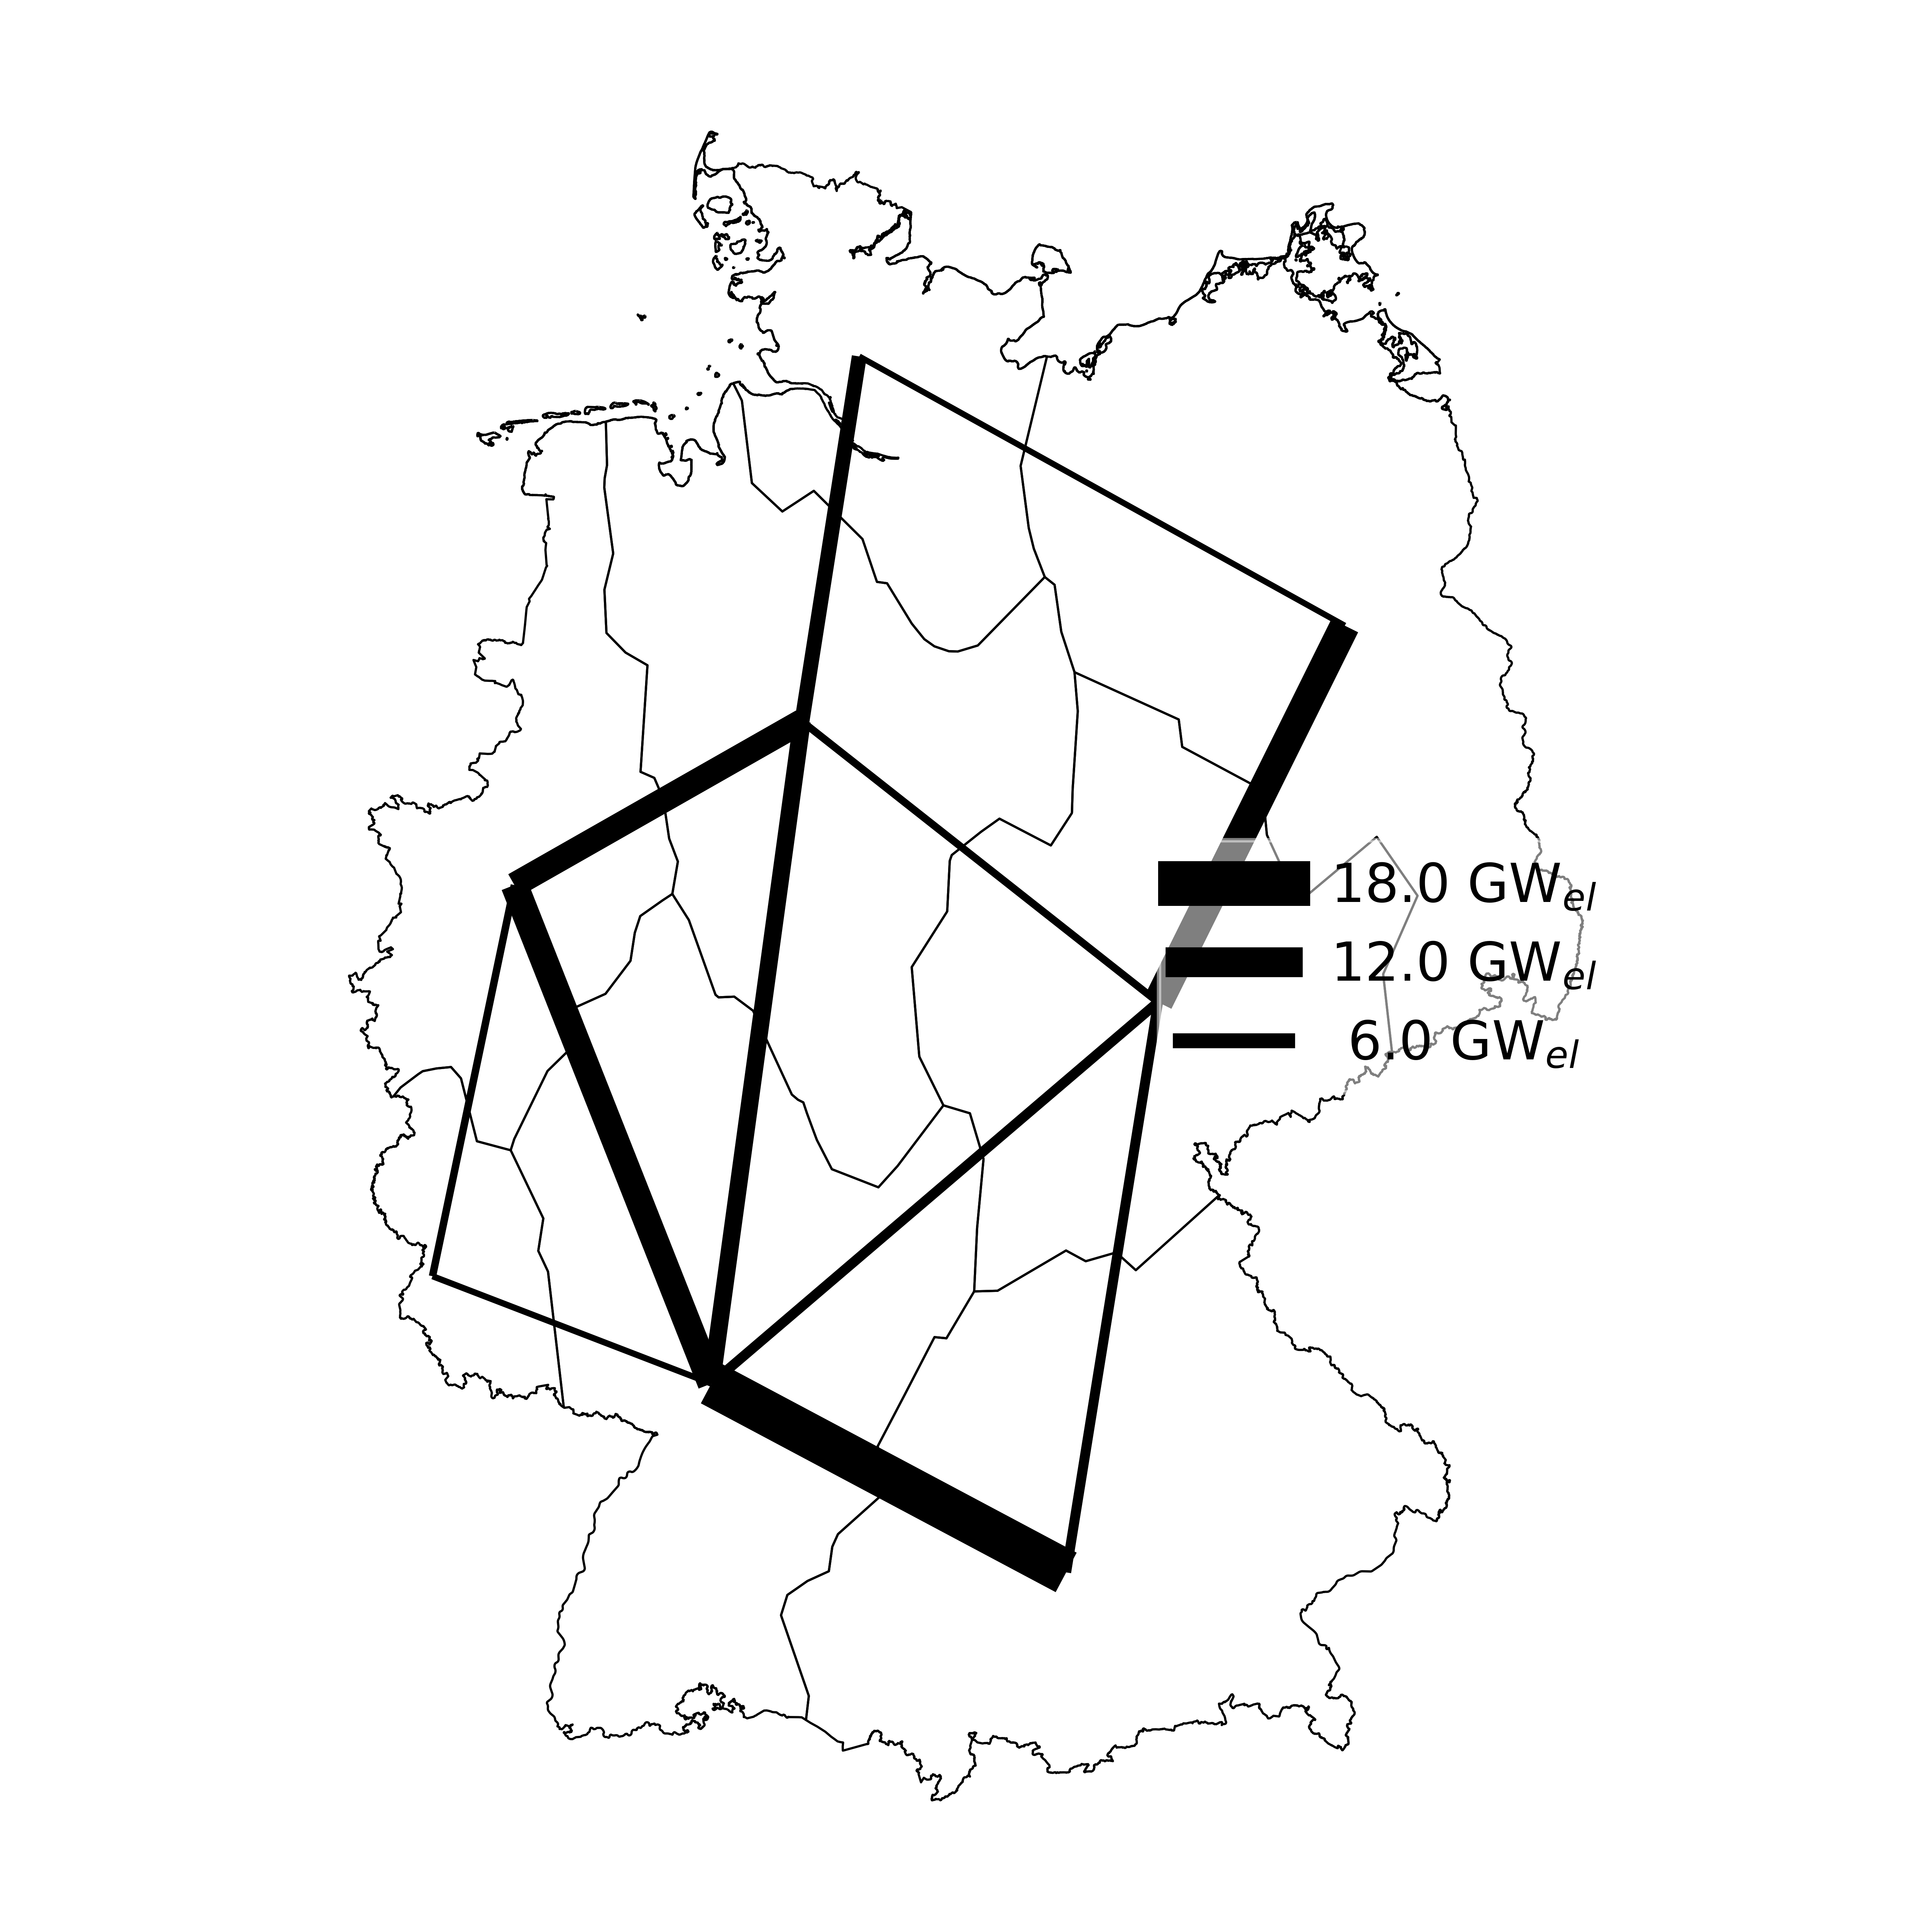
\includegraphics[width=\linewidth]{images/AC-insgesamt.png}
    \end{minipage}
    \hspace{.1\linewidth}
    \begin{minipage}[b]{.4\linewidth} 
       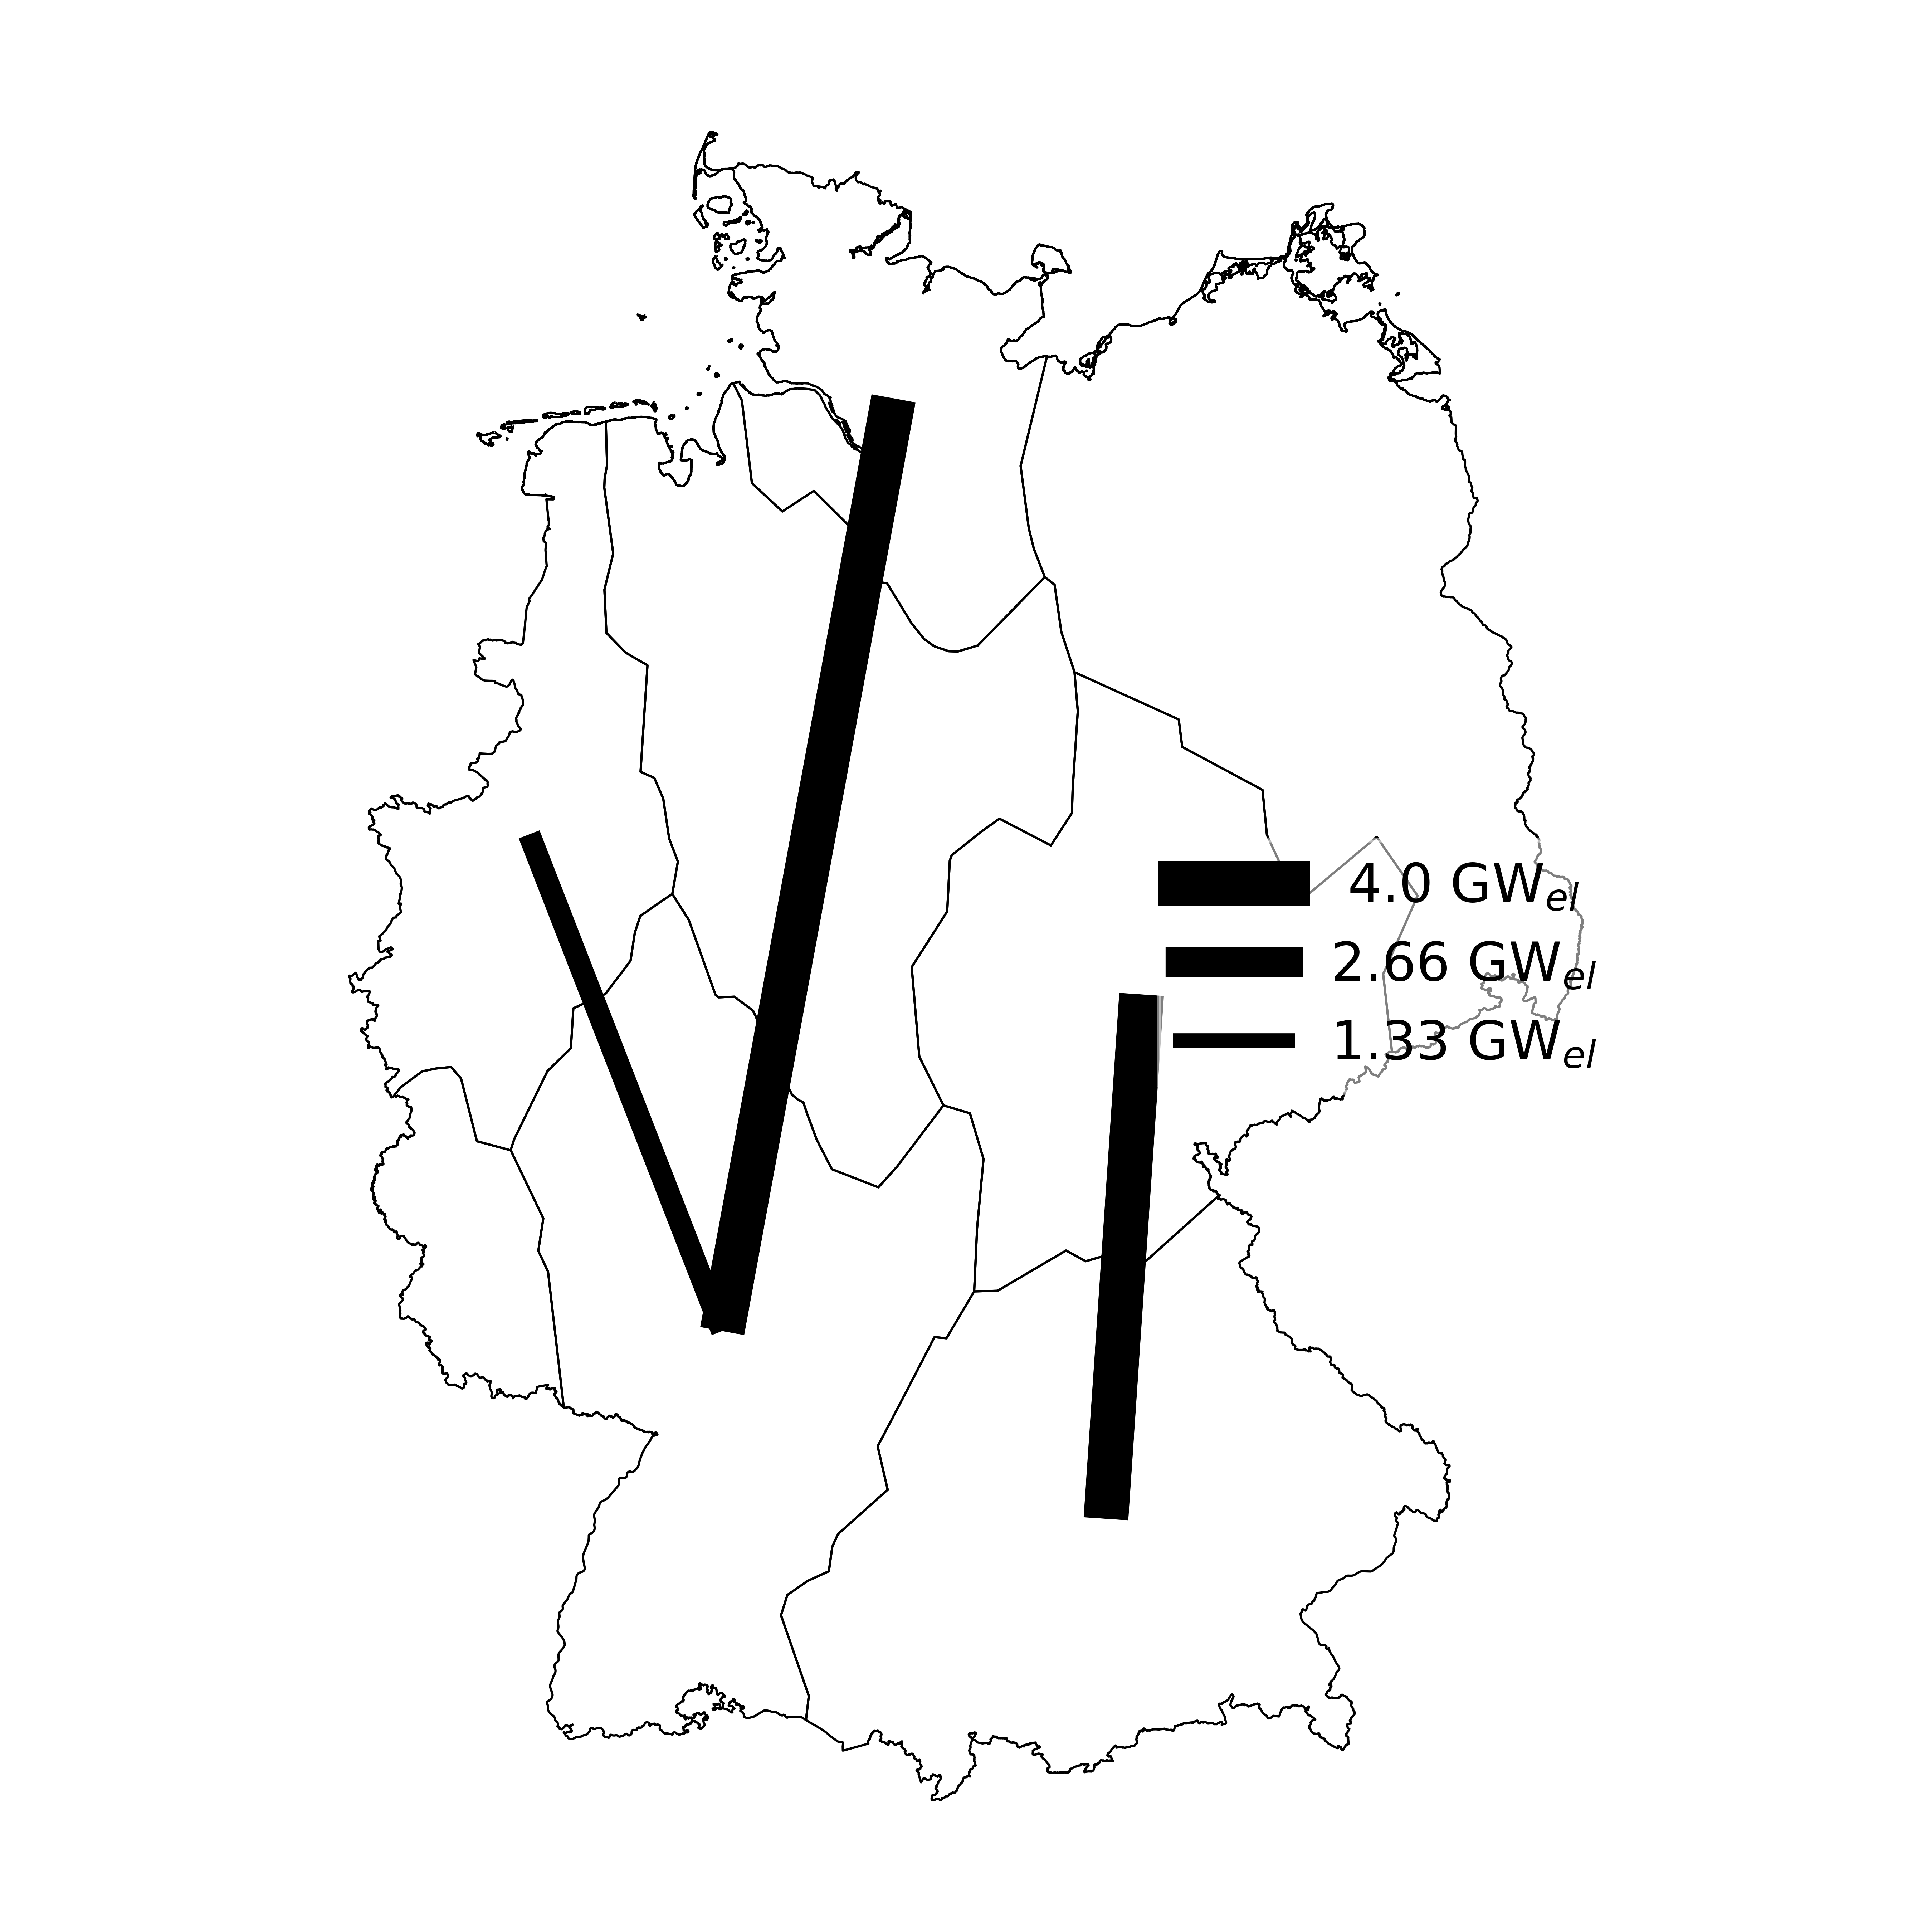
\includegraphics[width=\linewidth]{images/DC-insgesamt.png}
    \end{minipage}
    \caption{Lage der AC- und DC-Leitungen zwischen den acht Regionen}
    \label{image:Leitungen}
  \end{figure}


\subsection{Gesamtkosten (TAC)}
Für die Volkswirtschaft und die Zukunftsbetrachtung spielt die Kostenermittlung eine weitere Rolle. Als Kosten sind hier die Gesamtsystemkosten zu verstehen. Dabei handelt es sich im Wesentlichen um die fixen und variablen Betriebskosten, Investitionskosten und um die Importkosten. Im Rahmen der Projektarbeit und der zur Grunde liegenden Reduktionsfällen findet die Kostenoptimierung ebenfalls Berücksichtigung bei der Ausgestaltung des Energiemodells. Sollen Emissionswerte reduziert werden, impliziert dies die Einsparung fossiler Energieträger und führt somit zu einer Einsparung der Energiekosten. Berücksichtigt man alle für die Umsetzung erwähnten Komponenten für die unterschiedlichen Szenarien, belaufen sich die Gesamtkosten im 75 \% Fall auf ca. 41 Mrd. €/a und steigen im 100 \% Fall um 1,27 \% auf ca. 53 Mrd. €/a. Neben den Kosten für den Ausbau der Erzeugungsanlagen für erneuerbaren Energien, insbesondere Wind Offshore und Photovoltaik, stellt der Wechsel von Erdgas Verstromung zu Biogas den großen Anteil dar. Der Anteil der Kosten zur Energieerzeugung beträgt bei ungefähr bei jedem Reduktionsfall 85 \% der Gesamtsystemkosten. Eine genaue Kostenaufteilung ist der Abbildung \ref{image:TAC.png} zu entnehmen. 

\smallimage{TAC.png}{Aufteilung der Gesamtkosten für das Energiesystem nach Reduktionsfall}
